\documentclass[a4paper, 12pt]{article}

% ── Packages ────────────────────────────────────────────────────────────
\usepackage[utf8]{inputenc}
\usepackage[T1]{fontenc}
\usepackage[english]{babel}
\usepackage{geometry}
\geometry{margin=2.5cm}
\usepackage{graphicx}
\usepackage{hyperref}
\usepackage{xcolor}
\usepackage{listings}
\usepackage{tikz}
\usetikzlibrary{automata, positioning, arrows.meta}
\usepackage{enumitem}
\usepackage{booktabs}
\usepackage{amsmath}
\usepackage{parskip}

% ── Listings style ──────────────────────────────────────────────────────
\definecolor{codebg}{HTML}{F5F5F5}
\definecolor{codegreen}{HTML}{2E7D32}
\definecolor{codeblue}{HTML}{1565C0}
\definecolor{codegray}{HTML}{757575}

\lstset{
  backgroundcolor=\color{codebg},
  basicstyle=\ttfamily\small,
  keywordstyle=\color{codeblue}\bfseries,
  commentstyle=\color{codegray}\itshape,
  stringstyle=\color{codegreen},
  breaklines=true,
  frame=single,
  rulecolor=\color{codegray!40},
  numbers=left,
  numberstyle=\tiny\color{codegray},
  tabsize=4,
  showstringspaces=false
}

% ── Hyperref setup ──────────────────────────────────────────────────────
\hypersetup{
  colorlinks=true,
  linkcolor=codeblue,
  urlcolor=codeblue,
  citecolor=codeblue
}

% ── Title ───────────────────────────────────────────────────────────────
\title{%
  \textbf{Assignment \#03 --- Exercise 1} \\[0.3em]
  \Large Smart Home Alarm System \\[0.2em]
  \large Apache Pekko Actor-Based Implementation
}
\author{%
  Alessandro Martini \\
  \small Concurrent and Distributed Programming --- ISI LM \\
  \small University of Bologna, Cesena Campus
}
\date{A.Y.\ 2025--2026}

\begin{document}

\maketitle

% ═══════════════════════════════════════════════════════════════════════
\section{Problem Analysis}
% ═══════════════════════════════════════════════════════════════════════

The Smart Home Alarm System is a reactive control system that monitors a network of peripheral sensors (motion detectors, door/window contacts) and manages an alarm lifecycle through a well-defined finite state machine. Users interact with the system via a numeric keypad for arming, disarming, and alarm-silencing operations.

\subsection{Functional Overview}

The system operates through five states:

\begin{enumerate}[label=\arabic*.]
  \item \textbf{Disarmed} --- sensor events are ignored; normal house activity.
  \item \textbf{Exit Delay} --- countdown after arming; sensors still inactive so the user can leave.
  \item \textbf{Armed} --- sensors are active; any detection in an active zone triggers entry delay.
  \item \textbf{Entry Delay} --- countdown after intrusion detection; entering the correct PIN disarms the system.
  \item \textbf{Alarm} --- siren is active; only a correct PIN can silence it.
\end{enumerate}

The \emph{bonus} requirement extends the system with \textbf{zone-based partial arming}: the house is divided into zones (\texttt{LIVING\_AREA}, \texttt{SLEEPING\_AREA}, \texttt{PERIMETER}, \texttt{GROUND\_FLOOR}, \texttt{UPPER\_FLOOR}), and only sensors in \emph{active} zones can trigger the alarm.

\subsection{State Machine}

Figure~\ref{fig:fsm} illustrates the alarm state machine with all transitions.

\begin{figure}[ht]
  \centering
  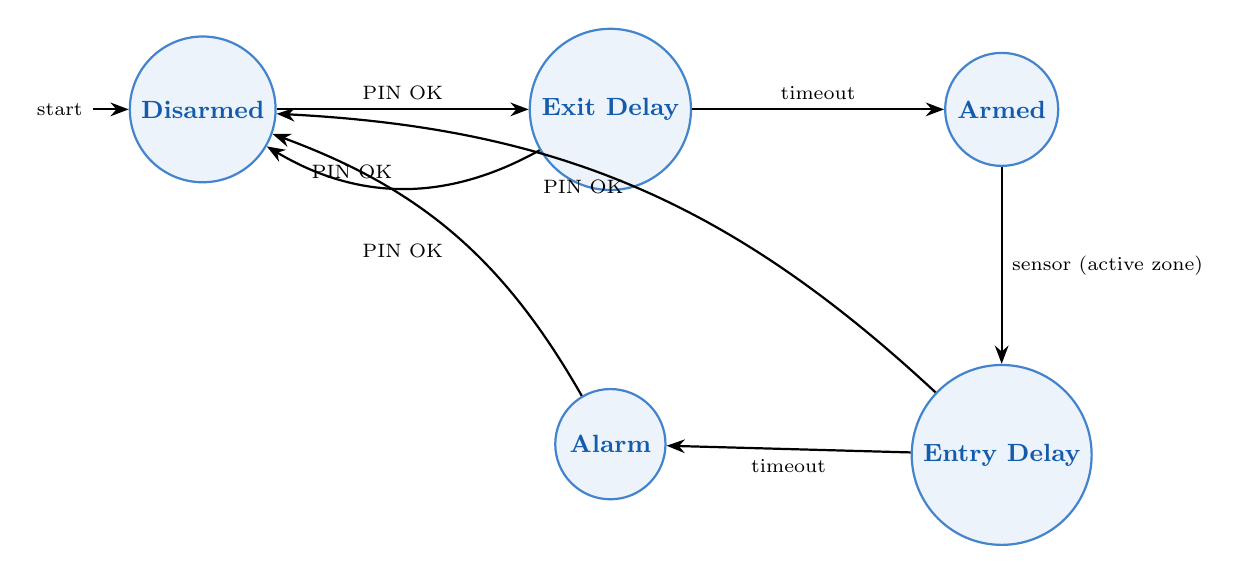
\begin{tikzpicture}[
    ->,
    >=Stealth,
    node distance=3.2cm,
    every state/.style={
      draw=codeblue!80,
      fill=codeblue!8,
      thick,
      minimum size=1.4cm,
      font=\small\bfseries,
      text=codeblue!90!black
    },
    every edge/.style={draw, thick, font=\scriptsize}
  ]
    \node[state, initial]           (D)   {Disarmed};
    \node[state, right=of D]        (EX)  {Exit Delay};
    \node[state, right=of EX]       (A)   {Armed};
    \node[state, below=2.5cm of A]  (EN)  {Entry Delay};
    \node[state, below=2.5cm of EX] (AL)  {Alarm};

    \path
      (D)  edge[above]                     node{PIN OK}            (EX)
      (EX) edge[above]                     node{timeout}           (A)
      (A)  edge[right]                     node{sensor (active zone)} (EN)
      (EN) edge[below]                     node{timeout}           (AL)
      (EN) edge[bend right=20, left]       node{PIN OK}            (D)
      (AL) edge[bend right=20, below left] node{PIN OK}            (D)
      (EX) edge[bend left=30, above left]  node{PIN OK}            (D);
  \end{tikzpicture}
  \caption{Finite state machine of the Smart Home Alarm System.}
  \label{fig:fsm}
\end{figure}

% ═══════════════════════════════════════════════════════════════════════
\section{Concurrency Analysis}
% ═══════════════════════════════════════════════════════════════════════

This problem is inherently concurrent: multiple sensors operate independently and simultaneously, a keypad accepts user input at any time, and timers fire asynchronously. Below we identify the key concurrent aspects and the challenges they pose.

\subsection{Sources of Concurrency}

\begin{description}[style=nextline]
  \item[Multiple Sensors]
    Each sensor (motion detector, door/window contact) is an independent entity that can fire events at any time. In a real deployment, dozens of sensors may trigger simultaneously, requiring the control unit to handle concurrent stimuli without data corruption or race conditions.

  \item[User Interaction]
    The keypad represents an additional concurrent input source. A user may enter a PIN while a sensor event is being processed, or during a timer countdown, creating interleaving scenarios that must be handled correctly.

  \item[Timer Management]
    Exit and entry delays are time-driven transitions. Timers run concurrently with message processing: a timer may expire while a PIN entry is being validated, or a sensor event may arrive during the last milliseconds of a countdown. These race conditions must be resolved deterministically.

  \item[State Consistency]
    The alarm state (\texttt{currentState}) and the set of active zones (\texttt{activeZones}) are mutable data that multiple concurrent events attempt to read or modify. Without proper isolation, concurrent access can lead to inconsistent states---e.g., processing a sensor event while the system is transitioning from \textsc{Exit Delay} to \textsc{Armed}.
\end{description}

\subsection{Concurrency Challenges}

\begin{enumerate}[label=\textbf{C\arabic*.}]
  \item \textbf{Race between timer expiration and user input.} If the entry delay timer expires at the same instant the user enters a correct PIN, the outcome must be deterministic: either the system disarms or the alarm triggers, but not both.
  \item \textbf{Simultaneous sensor events.} Multiple sensors may fire at the same time. The system must ensure that only the first event in \textsc{Armed} state triggers the entry delay; subsequent events should have no additional effect.
  \item \textbf{Timer cancellation.} When the user disarms during a delay phase, the pending timer must be reliably cancelled. Failure to do so could cause a spurious transition after disarming.
  \item \textbf{Zone set mutation.} Switching between full and partial arming modifies the active zone set. This mutation must not interfere with concurrent sensor-event evaluation.
\end{enumerate}

% ═══════════════════════════════════════════════════════════════════════
\section{Adopted Strategy}
% ═══════════════════════════════════════════════════════════════════════

The system is implemented using the \textbf{Actor Model}, specifically the \textbf{Apache Pekko} framework (typed API, Java). The actor model is a natural fit for this problem because it provides \emph{message-driven concurrency with encapsulated state}, resolving all the challenges identified above.

\subsection{Architecture Overview}

The system is decomposed into three actor types:

\begin{table}[ht]
  \centering
  \begin{tabular}{@{} l l p{7.5cm} @{}}
    \toprule
    \textbf{Actor} & \textbf{Protocol} & \textbf{Responsibility} \\
    \midrule
    \texttt{AlarmSystem}  & \texttt{AlarmCommand} & Central control unit: implements the FSM, manages timers, validates PINs, and emits events. \\
    \texttt{Sensor}       & \texttt{Sensor.Command} & Represents a physical sensor. On trigger, sends a \texttt{SensorEvent} to the alarm system. \\
    \texttt{EventLogger}  & \texttt{AlarmEvent} & Subscribes to alarm events for logging/auditing purposes. \\
    \bottomrule
  \end{tabular}
  \caption{Actor decomposition.}
  \label{tab:actors}
\end{table}

\subsection{Why the Actor Model Solves the Concurrency Challenges}

\begin{description}[style=nextline]
  \item[Single-threaded message processing (mailbox)]
    Each actor processes \emph{one message at a time} from its mailbox. This sequential processing within the \texttt{AlarmSystem} actor eliminates all race conditions on \texttt{currentState} and \texttt{activeZones}---no locks, no synchronization, no shared mutable state. Concurrent sensor events and user commands are serialized by the mailbox.

  \item[Timer integration via \texttt{TimerScheduler}]
    Pekko's \texttt{TimerScheduler} delivers timer expirations as regular messages into the actor's mailbox. This means timer callbacks are \emph{interleaved with other messages} in a deterministic, sequential order. If a \texttt{DisarmSystem} message arrives before \texttt{ExitDelayTimeout}, the disarm is processed first, the timer is cancelled, and the timeout message (if delivered) is harmlessly ignored because the state guard check fails.

  \item[Location transparency and isolation]
    Sensor actors communicate with the \texttt{AlarmSystem} exclusively through \texttt{ActorRef<AlarmCommand>} references. There is no shared memory between actors. Each sensor is a self-contained entity that can be spawned, stopped, or relocated independently.

  \item[Typed protocols]
    The use of Pekko's typed API with sealed interfaces (\texttt{AlarmCommand}, \texttt{AlarmEvent}) ensures at compile time that actors only receive messages they can handle, reducing the risk of protocol violations.
\end{description}

\subsection{Key Design Decisions}

\subsubsection{State Machine as Conditional Logic}

Rather than using Pekko's behavior-switching pattern (where each state is a separate \texttt{Behavior}), the implementation uses a single behavior with a \texttt{currentState} field and guard conditions on each message handler. This was chosen for simplicity: the state machine has only five states and the transition logic benefits from being in one cohesive place.

\begin{lstlisting}[language=Java, caption={Guard-based state handling (excerpt).}]
private Behavior<AlarmCommand> onSensorEvent(SensorEvent cmd) {
    if (currentState == State.DISARMED
            || currentState == State.EXIT_DELAY) {
        return Behaviors.same(); // ignore
    }
    if (currentState == State.ARMED
            && activeZones.contains(cmd.zone())
            && cmd.triggered()) {
        startEntryDelay(cmd.zone());
    }
    return Behaviors.same();
}
\end{lstlisting}

\subsubsection{Timer Keys for Reliable Cancellation}

Each timer is associated with a named key (\texttt{EXIT\_TIMER\_KEY}, \texttt{ENTRY\_TIMER\_KEY}). When the user disarms or re-arms, the corresponding timer is explicitly cancelled via \texttt{timers.cancel(key)}, preventing stale timeout messages from causing spurious transitions.

\subsubsection{Zone-Based Partial Arming (Bonus)}

Zones are modelled as a Java \texttt{EnumSet<Zone>}. Full arming activates \texttt{EnumSet.allOf(Zone.class)}, while partial arming uses a user-specified subset. Sensor events are filtered against \texttt{activeZones} before triggering transitions, enabling scenarios such as \emph{night mode} (perimeter and ground floor active, upper floor inactive).

\subsection{Message Flow}

The typical interaction flow for an intrusion scenario is:

\begin{enumerate}
  \item \textbf{User $\rightarrow$ AlarmSystem}: \texttt{ArmSystem("1234")} or \texttt{ArmSystemPartial("1234", zones)}
  \item \textbf{AlarmSystem}: validates PIN, transitions to \textsc{Exit Delay}, starts exit timer
  \item \textbf{Timer $\rightarrow$ AlarmSystem}: \texttt{ExitDelayTimeout} $\Rightarrow$ transition to \textsc{Armed}
  \item \textbf{Sensor $\rightarrow$ AlarmSystem}: \texttt{SensorEvent(MOTION, LIVING\_AREA, true)}
  \item \textbf{AlarmSystem}: zone is active $\Rightarrow$ transition to \textsc{Entry Delay}, starts entry timer
  \item \textbf{Timer $\rightarrow$ AlarmSystem}: \texttt{EntryDelayTimeout} $\Rightarrow$ transition to \textsc{Alarm}
  \item \textbf{User $\rightarrow$ AlarmSystem}: \texttt{StopAlarm("1234")} $\Rightarrow$ transition to \textsc{Disarmed}
\end{enumerate}

All steps occur through asynchronous message passing, with the mailbox guaranteeing sequential processing and state consistency.

\subsection{Testing Strategy}

The system is tested using \textbf{Pekko ActorTestKit} with \texttt{TestProbe} instances acting as event sinks. The test suite covers:

\begin{itemize}
  \item Full arming lifecycle (Disarmed $\rightarrow$ Exit Delay $\rightarrow$ Armed)
  \item Intrusion sequence (Armed $\rightarrow$ Entry Delay $\rightarrow$ Alarm)
  \item Disarming during entry delay (race condition scenario)
  \item Disarming during exit delay (timer cancellation)
  \item Invalid PIN rejection at each state
  \item Sensor events ignored in Disarmed and Exit Delay states
  \item Zone-based filtering: inactive zones ignored, active zones trigger correctly
  \item Partial arming with mixed active/inactive zones
\end{itemize}

% ═══════════════════════════════════════════════════════════════════════
\section{Conclusions}
% ═══════════════════════════════════════════════════════════════════════

The actor model, as implemented via Apache Pekko, proved to be an excellent paradigm for the Smart Home Alarm System. The key insight is that the actor's mailbox provides a natural serialization point that eliminates the need for explicit synchronization, while timer messages are seamlessly integrated into the same sequential message flow. This design yields a system that is both \emph{correct by construction} with respect to concurrency and \emph{easy to reason about}, since the entire state machine logic resides within a single actor processing one message at a time.

\end{document}
